\documentclass{article}
\usepackage{amsmath}
\usepackage{amssymb}
\usepackage{parallel}
\usepackage[most]{tcolorbox}
\usepackage{amsthm}
\usepackage[a4paper,
top=1.5cm,
bottom=1.5cm,
left=1.8cm,
right=1.8cm,
heightrounded]
{geometry}
\renewcommand{\arraystretch}{2.5}

\title{QF 620 \protect \\ Stochastic Modelling in Finance\\
	\textbf{Project Report}}

\date{}

\begin{document}
	
% PART 1: BLACK SCHOLES %%%%%%%%%%%%%%%%%%%%%%%%%%%%%%%%%%%%%%%%%%%%%%%%
\section*{Part I: Analytical Option Formulae}
\section{The Black-Scholes Model}
\begin{minipage}[t]{0.5\textwidth}
	\begin{tcolorbox}[height=11.5cm,boxsep=5pt,arc=0pt,auto outer arc,colback=white,colframe=black]
		\noindent \textbf{Solving SDE}\\ \\
		\noindent Given that: $\boldsymbol{dS_t = r S_t dt + \sigma S_t dW_t}$\\ \\
		\noindent Let: $X_t = \log (S_t) = f(S_t)$\\ \\
		\noindent By Itô's Formula:
		\begin{align*}
		dX_t &= f'(S_t) dS_t + \frac{1}{2} f''(S_t) (dS_t)^2\\
		&= \frac{1}{S_t} (r S_t dt + \sigma S_t dW_t) - \frac{1}{2} \frac{1}{S_t^2} (\sigma^2 S_t^2 dt)\\
		&= \left(r-\frac{1}{2} \sigma^2 \right) dt + \sigma dW_t
		\end{align*}
		\noindent Integrating:
		\begin{flalign*}
		\int_{0}^{T} dX_t &= \left(r-\frac{1}{2} \sigma^2 \right) \int_{0}^{T} dt +  \sigma \int_{0}^{T} dW_t\\
		\log \left( \frac{S_T}{S_0} \right) &= \left(r-\frac{1}{2} \sigma^2 \right)T + \sigma W_T\\
		\boldsymbol{S_T }&\boldsymbol{= S_0 \exp\left[ \left(r-\frac{1}{2} \sigma^2 \right)T + \sigma W_T \right]}
		\end{flalign*}
		\noindent where $W_T \sim N(0,T) \sim \sqrt{T} N(0,1) \sim \sqrt{T} x$.
	\end{tcolorbox}
\end{minipage}
\begin{minipage}[t]{0.5\textwidth}
	\begin{tcolorbox}[height=11.5cm,boxsep=5pt,arc=0pt,auto outer arc,colback=white,colframe=black]
		\noindent \textbf{Finding $\boldsymbol{x^*}$ where $\boldsymbol{S_T=K}$}
		\begin{flalign*}
		S_T &= K\\
		K &= S_0 \exp\left[ \left(r-\frac{1}{2} \sigma^2 \right)T + \sigma \sqrt{T} x \right]\\
		\log \left( \frac{K}{S_0} \right) &= \left(r-\frac{1}{2} \sigma^2 \right)T + \sigma \sqrt{T} x\\
		\boldsymbol{x^* }&\boldsymbol{= \frac{\log\left( \frac{K}{S_0} \right) - \left( r-\frac{\sigma^2}{2} \right)T}{\sigma \sqrt{T}}}
		\end{flalign*}
		\noindent \textbf{Additional Comments}\\ 
		In the Black Scholes option pricing model, the valuation of the underlying asset is valued using a risk-neutral probability framework where the asset's prices are expressed  with a risk-free bond used as the numeraire security. \\ \\
	    As a result, the relative price process is turned into a martingale as the asset price process' previous drift term $\mu$ is replaced by the risk-free rate $r$.\\ \\
		With the stock price process (discounted by the risk-free bond) expressed as a martingale, arbitrage opportunities are also eliminated.
	\end{tcolorbox}
\end{minipage} \\ \\
\noindent \textbf{Derivation for Vanilla Call ($\boldsymbol{V_0^c}$) and Put ($\boldsymbol{V_0^p}$) Option Valuation Formulae}
\begin{flalign*}
V_0^c&=e^{-rT}\mathbb{E}[(S_T-K)^+]\\
&=e^{-rT}\left[ \int_{x^*}^{\infty} \frac{1}{\sqrt{2\pi}}\left( S_0 e^{\left(r-\frac{\sigma^2}{2}\right)T+\sigma \sqrt{T} x} - K\right)e^{-\frac{x^2}{2}} dx \right]\\
&=e^{-rT}\left[ S_0 e^{\left(r-\frac{\sigma^2}{2}\right)T}  \int_{x^*}^{\infty} \frac{1}{\sqrt{2\pi}} e^{-\frac{x^2-2 \sigma \sqrt{T} x + \sigma^2 T - \sigma^2 T}{2}} dx - K \int_{x^*}^{\infty} \frac{1}{\sqrt{2\pi}} e^{-\frac{x^2}{2}} dx\right]\\
&=e^{-rT}\left[ S_0 e^{rT} \int_{x^*}^{\infty} \frac{1}{\sqrt{2\pi}} e^{-\frac{(x-\sigma \sqrt{T})^2}{2}} dx - K \int_{x^*}^{\infty} \frac{1}{\sqrt{2\pi}} e^{-\frac{x^2}{2}} dx \right]\\
&= e^{-rT}\left[ S_0 e^{rT} \Phi (-x^* + \sigma \sqrt{T}) - K \Phi (-x^*) \right]\\
\boldsymbol{V_0^c }&\boldsymbol{= \boldsymbol{S_0 \Phi \left( \frac{\log\left( \frac{S_0}{K} \right) + \left( r+\frac{\sigma^2}{2} \right)T}{\sigma \sqrt{T}} \right) - K e^{-rT} \Phi \left( \frac{\log\left( \frac{S_0}{K} \right) + \left( r-\frac{\sigma^2}{2} \right)T}{\sigma \sqrt{T}} \right)}}\\
\boldsymbol{V_0^p }&\boldsymbol{=K e^{-rT} \Phi \left( \frac{\log\left( \frac{K}{S_0} \right) - \left( r-\frac{\sigma^2}{2} \right)T}{\sigma \sqrt{T}} \right) - S_0 \Phi \left( \frac{\log\left( \frac{K}{S_0} \right) - \left( r+\frac{\sigma^2}{2} \right)T}{\sigma \sqrt{T}} \right)}
\end{flalign*}\\
\noindent \textbf{Valuation Formulae for Other Option Types}
\\
\begin{center}
	\begin{tabular}{|c|c|c|}
		\hline
		\textbf{Option Type}& \textbf{Call} & \textbf{Put}\\
		\hline
		Digital Cash-or-Nothing&
		$e^{-rT} \Phi \left( \frac{\log\left( \frac{S_0}{K} \right) + \left( r-\frac{\sigma^2}{2} \right)T}{\sigma \sqrt{T}} \right)$&
		$e^{-rT} \Phi \left( \frac{\log\left( \frac{K}{S_0} \right) - \left( r-\frac{\sigma^2}{2} \right)T}{\sigma \sqrt{T}} \right)$
		\\
		\hline
		Digital Asset-or-Nothing& 
		$S_0 \Phi \left( \frac{\log\left( \frac{S_0}{K} \right) + \left( r+\frac{\sigma^2}{2} \right)T}{\sigma \sqrt{T}} \right)$&
		$S_0 \Phi \left( \frac{\log\left( \frac{K}{S_0} \right) - \left( r+\frac{\sigma^2}{2} \right)T}{\sigma \sqrt{T}} \right)$
		\\
		\hline
	\end{tabular}
\end{center}

\newpage

% PART 1: BLACK76 LOGNORMAL %%%%%%%%%%%%%%%%%%%%%%%%%%%%%%%%%%%%%%%%%%%%

\section{The Black76 Lognormal Model}
\begin{minipage}[t]{0.5\textwidth}
	\begin{tcolorbox}[height=12.4cm,boxsep=5pt,arc=0pt,auto outer arc,colback=white,colframe=black]
		\noindent \textbf{Solving SDE}\\ \\
		\noindent Given that: $\boldsymbol{dF_t = \sigma F_t dW_t}$\\ \\
		\noindent Let: $X_t = \log (F_t) = f(F_t)$\\ \\
		\noindent where $F_T = S_T e^{rT}$.\\ \\
		\noindent By Itô's Formula:
		\begin{align*}
		dX_t &= f'(F_t) dF_t + \frac{1}{2} f''(F_t) (dF_t)^2\\
		&= \frac{1}{F_t} (\sigma F_t dW_t) - \frac{1}{2} \frac{1}{F_t^2} (\sigma^2 F_t^2 dt)\\
		&= -\frac{1}{2} \sigma^2 dt + \sigma dW_t
		\end{align*}
		\noindent Integrating:
		\begin{flalign*}
		\int_{0}^{T} dX_t &= - \frac{1}{2} \sigma^2 \int_{0}^{T} dt +  \sigma \int_{0}^{T} dW_t\\
		\log \left( \frac{F_T}{F_0} \right) &= -\frac{1}{2} \sigma^2 T + \sigma W_T\\
		\boldsymbol{F_T }&\boldsymbol{= F_0 \exp\left[ -\frac{1}{2} \sigma^2 T + \sigma W_T \right]}
		\end{flalign*}
		\noindent where $W_T \sim N(0,T) \sim \sqrt{T} N(0,1) \sim \sqrt{T} x$.
	\end{tcolorbox}
\end{minipage}
\begin{minipage}[t]{0.5\textwidth}
	\begin{tcolorbox}[height=12.4cm,boxsep=5pt,arc=0pt,auto outer arc,colback=white,colframe=black]
		\noindent \textbf{Finding $\boldsymbol{x^*}$ where $\boldsymbol{F_T=K}$}
		\begin{flalign*}
		F_T &= K\\
		K &= F_0 \exp\left[ -\frac{1}{2} \sigma^2 T + \sigma \sqrt{T} x \right]\\
		\log \left( \frac{K}{F_0} \right) &= -\frac{1}{2} \sigma^2 T + \sigma \sqrt{T} x\\
		\boldsymbol{x^* }&\boldsymbol{= \frac{\log\left( \frac{K}{F_0} \right) + \frac{\sigma^2 T}{2}}{\sigma \sqrt{T}}}
		\end{flalign*}\\
		\noindent \textbf{Additional Comments}\\ \\
		The Black76 Lognormal model is structurally identical to the Black-Scholes model but with forward prices, as opposed to stock prices, used instead. An advantage of using forward prices instead of stock prices is that the SDE for forward prices is more compact, driftless and is therefore a martingale.\\ \\
		Also, when using the Black76 model, the interest rate $r$ is not required for the computation of expected future option values. All inputs being constant, the Black-Scholes model and the Black76 Lognormal model should suggest at the same option values.
	\end{tcolorbox}
\end{minipage}\\ 

\noindent \textbf{Derivation for Vanilla Call ($\boldsymbol{V_0^c}$) and Put ($\boldsymbol{V_0^p}$) Option Valuation Formulae}
\begin{flalign*}
V_0^c&=e^{-rT}\mathbb{E}[(F_T-K)^+]\\
&=e^{-rT}\left[ \int_{x^*}^{\infty} \frac{1}{\sqrt{2\pi}}\left( F_0 e^{\left( -\frac{\sigma^2 T}{2} + \sigma \sqrt{T} x \right)} - K\right)e^{-\frac{x^2}{2}} dx \right]\\
&=e^{-rT}\left[ F_0 e^{-\frac{\sigma^2 T}{2}} \int_{x^*}^{\infty} \frac{1}{\sqrt{2\pi}} e^{-\frac{x^2-2 \sigma \sqrt{T} x + \sigma^2 T - \sigma^2 T}{2}} dx - K \int_{x^*}^{\infty} \frac{1}{\sqrt{2\pi}} e^{-\frac{x^2}{2}} dx\right]\\
&=e^{-rT}\left[ F_0 \int_{x^*}^{\infty} \frac{1}{\sqrt{2\pi}} e^{-\frac{(x-\sigma \sqrt{T})^2}{2}} dx - K \int_{x^*}^{\infty} \frac{1}{\sqrt{2\pi}} e^{-\frac{x^2}{2}} dx \right]\\
&= e^{-rT}\left[ F_0 \Phi (-x^* + \sigma \sqrt{T}) - K \Phi (-x^*) \right]\\
\boldsymbol{V_0^c }&\boldsymbol{= e^{-rT}\left[F_0 \Phi \left( \frac{\log\left( \frac{F_0}{K} \right) + \frac{\sigma^2 T}{2}}{\sigma \sqrt{T}} \right) - K \Phi \left( \frac{\log\left( \frac{F_0}{K} \right) - \frac{\sigma^2 T}{2}}{\sigma \sqrt{T}}  \right) \right]}\\
\boldsymbol{V_0^p }&\boldsymbol{=e^{-rT}\left[K \Phi \left(  \frac{\log\left( \frac{K}{F_0} \right) + \frac{\sigma^2 T}{2}}{\sigma \sqrt{T}} \right) - F_0 \Phi \left( \frac{\log\left( \frac{K}{F_0} \right) - \frac{\sigma^2 T}{2}}{\sigma \sqrt{T}} \right) \right]}
\end{flalign*}\\
\noindent \textbf{Valuation Formulae for Other Option Types}
\\
\begin{center}
	\begin{tabular}{|c|c|c|}
		\hline
		\textbf{Option Type}& \textbf{Call} & \textbf{Put}\\
		\hline
		Digital Cash-or-Nothing&
		$e^{-rT} \Phi \left( \frac{\log\left( \frac{F_0}{K} \right) - \frac{\sigma^2 T}{2}}{\sigma \sqrt{T}} \right)$&
		$e^{-rT} \Phi \left( \frac{\log\left( \frac{K}{F_0} \right) + \frac{\sigma^2 T}{2}}{\sigma \sqrt{T}} \right)$
		\\
		\hline
		Digital Asset-or-Nothing& 
		$e^{-rT} F_0 \Phi \left( \frac{\log\left( \frac{F_0}{K} \right) + \frac{\sigma^2 T}{2}}{\sigma \sqrt{T}} \right)$&
		$e^{-rT} F_0 \Phi \left( \frac{\log\left( \frac{K}{F_0} \right) - \frac{\sigma^2 T}{2}}{\sigma \sqrt{T}} \right)$
		\\
		\hline
	\end{tabular}
\end{center}

\newpage

% PART 1: BACHELIER & BLACK76 NORMAL %%%%%%%%%%%%%%%%%%%%%%%%%%%%%%%%%%%%%%%%%%

\section{The Bachelier \& the Black76 Normal Model}
\noindent Structurally, the Bachelier and the Black76 Normal models are very similar. Derivations will be shown side-by-side to highlight their structural similarities.\\ \\
\begin{minipage}[t]{0.5\textwidth}
	\begin{tcolorbox}[height=10.1cm,boxsep=5pt,arc=0pt,auto outer arc,colback=white,colframe=black]
		\noindent \textbf{The Bachelier Model}\\ \\
		\noindent \textbf{Solving SDE}\\ \\
		\noindent Given that: $\boldsymbol{dS_t = \sigma S_t dW_t}$\\ \\
		\noindent Integrating:
		\begin{flalign*}
		\int_{0}^{T} dS_t &= \sigma S_0 \int_{0}^{T} dW_t\\
		S_T - S_0 &= \sigma S_0 W_T\\
		\boldsymbol{S_T }&\boldsymbol{= S_0(1 + \sigma W_T)}
		\end{flalign*}
		\noindent where $W_T \sim N(0,T) \sim \sqrt{T} N(0,1) \sim \sqrt{T} x$.\\ \\
		\noindent \textbf{Finding $\boldsymbol{x^*}$ where $\boldsymbol{S_T=K}$}
		\begin{flalign*}
		S_T &= K\\
		K &= S_0 + S_0 \sigma \sqrt{T} x\\
		\boldsymbol{x^* } & \boldsymbol{= \frac{K-S_0}{S_0 \sigma \sqrt{T}}}
		\end{flalign*}
	\end{tcolorbox}
\end{minipage}
\begin{minipage}[t]{0.5\textwidth}
	\begin{tcolorbox}[height=10.1cm,boxsep=5pt,arc=0pt,auto outer arc,colback=white,colframe=black]
		\noindent \textbf{The Black76 Normal Model}\\ \\
		\noindent \textbf{Solving SDE}\\ \\
		\noindent Given that: $\boldsymbol{dF_t = \sigma F_t dW_t}$\\ \\
		\noindent Integrating:
		\begin{flalign*}
		\int_{0}^{T} dF_t &= \sigma F_0 \int_{0}^{T} dW_t\\
		F_T - F_0 &= \sigma F_0 W_T\\
		\boldsymbol{F_T }&\boldsymbol{= F_0(1 + \sigma W_T)}
		\end{flalign*}
		\noindent where $W_T \sim N(0,T) \sim \sqrt{T} N(0,1) \sim \sqrt{T} x$.\\ \\
		\noindent \textbf{Finding $\boldsymbol{x^*}$ where $\boldsymbol{F_T=K}$}
		\begin{flalign*}
		F_T &= K\\
		K &= F_0 + F_0 \sigma \sqrt{T} x\\
		\boldsymbol{x^* } & \boldsymbol{= \frac{K-F_0}{F_0 \sigma \sqrt{T}}}
		\end{flalign*}
	\end{tcolorbox}
\end{minipage}\\ 

\noindent \textbf{Derivation for Vanilla Call ($\boldsymbol{V_0^c}$) and Put ($\boldsymbol{V_0^p}$) Option Valuation Formulae for Bachelier Model}\\ \\
\noindent Given the similarity in structure between the Bachelier and the Black76 Normal models, the option valuation formulae for the Black76 Normal model can be obtained simply by replacing the $\boldsymbol{S_T}$ and $\boldsymbol{S_0}$ terms in the Bachelier option valuation formulae with $\boldsymbol{F_T}$ and $\boldsymbol{F_0}$ respectively.
\begin{flalign*}
V_0^c&=e^{-rT}\mathbb{E}[(S_T-K)^+]\\
&=e^{-rT}\left[ \int_{x^*}^{\infty} \frac{1}{\sqrt{2\pi}}\left( S_0 + S_0 \sigma \sqrt{T} x - K\right) e^{-\frac{x^2}{2}} dx \right]\\
&=e^{-rT}\left[(S_0-K)\int_{x^*}^{\infty} \frac{1}{\sqrt{2\pi}} e^{-\frac{x^2}{2}} dx + S_0 \sigma \sqrt{T} \int_{x^*}^{\infty} x \cdot e^{-\frac{x^2}{2}} dx \right]\\
&=e^{-rT}\left[ (S_0-K)\int_{x^*}^{\infty} \frac{1}{\sqrt{2\pi}} e^{-\frac{x^2}{2}} dx - S_0 \sigma \sqrt{T} \int_{x^*}^{\infty} e^u du\right]\\
&=e^{-rT}\left[ (S_0-K)\int_{x^*}^{\infty} \frac{1}{\sqrt{2\pi}} e^{-\frac{x^2}{2}} dx - S_0 \sigma \sqrt{T} \left[ e^{-\frac{x^2}{2}}\right]^{\infty}_{x^*} \right]\\
&=e^{-rT}\left[ (S_0-K) \Phi (-x^*) + S_0 \sigma \sqrt{T} \phi (-x^*) \right]\\
\boldsymbol{V_0^c} &=\boldsymbol{e^{-rT}\left[ (S_0-K) \Phi \left(\frac{S_0-K}{S_0 \sigma \sqrt{T}}\right) + S_0 \sigma \sqrt{T} \phi \left(\frac{S_0-K}{S_0 \sigma \sqrt{T}}\right) \right]}\\
\boldsymbol{V_0^p} &=\boldsymbol{e^{-rT}\left[ (K-S_0) \Phi \left(\frac{K-S_0}{S_0 \sigma \sqrt{T}}\right) + S_0 \sigma \sqrt{T} \phi \left(\frac{K-S_0}{S_0 \sigma \sqrt{T}}\right) \right]}
\end{flalign*}\\
\noindent \textbf{Valuation Formulae for Other Option Types}
\\
\begin{center}
	\begin{tabular}{|c|c|c|}
		\hline
		\textbf{Option Type}& \textbf{Call} & \textbf{Put}\\
		\hline
		Digital Cash-or-Nothing&
		$e^{-rT} \Phi \left( \frac{S_0-K}{S_0 \sigma \sqrt{T}} \right)$&
		$e^{-rT} \Phi \left( \frac{K-S_0}{S_0 \sigma \sqrt{T}} \right)$
		\\
		\hline
		Digital Asset-or-Nothing& 
		$e^{-rT} S_0 \left[\Phi \left( \frac{S_0-K}{S_0 \sigma \sqrt{T}} \right) + \sigma \sqrt{T} \phi \left( \frac{S_0-K}{S_0 \sigma \sqrt{T}} \right)\right]$&
		$e^{-rT} S_0 \left[\Phi \left( \frac{K-S_0}{S_0 \sigma \sqrt{T}} \right) - \sigma \sqrt{T} \phi \left( \frac{K-S_0}{S_0 \sigma \sqrt{T}} \right)\right]$
		\\
		\hline
	\end{tabular}
\end{center}

\newpage

% PART 1: DISPLACED DIFFUSION %%%%%%%%%%%%%%%%%%%%%%%%%%%%%%%%%%%%%%%%%%%%%%%%

\section{The Displaced Diffusion (DD) Model}
\begin{minipage}[t]{0.58\textwidth}
	\begin{tcolorbox}[height=15.5cm,boxsep=5pt,arc=0pt,auto outer arc,colback=white,colframe=black]
		\noindent \textbf{Solving SDE}\\ \\
		\noindent Given that: $\boldsymbol{dF_t=\sigma [ \beta F_t + (1 - \beta) F_0 ] dW_t}$\\ \\
		\noindent Let: $X_t = \log (\beta F_t + (1- \beta) F_0) = f(F_t)$\\ \\
		\noindent By Itô's formula: 
		\begin{flalign*}
		dX_t&=f'(F_t)dF_t + \frac{1}{2} f''(F_t)(dF_t)^2\\
		&=\frac{\beta}{\beta F_t + (1- \beta) F_0}(\sigma (\beta F_t + (1 - \beta) F_0) dW_t)\\
		& - \frac{1}{2}\frac{\beta^2}{(\beta F_t + (1- \beta) F_0)^2}(\sigma^2 (\beta F_t + (1 - \beta) F_0)^2 d_t)\\
		&= \beta \sigma dW_t - \frac{1}{2} \beta^2 \sigma^2 dt
		\end{flalign*}
		\noindent Integrating:\\
		\begin{flalign*}
		\int_{0}^{T} dX_t &= \beta \sigma \int_{0}^{T} dW_t - \frac{1}{2} \beta^2 \sigma^2 \int_{0}^{T} dt\\
		X_T - X_0 &= \beta \sigma W_T - \frac{1}{2} \beta^2 \sigma^2 T\\
		\log \left( \frac{\beta F_T + (1 - \beta) F_0}{\beta F_0 + (1 - \beta) F_0} \right) &= \beta \sigma W_T - \frac{1}{2} \beta^2 \sigma^2 T\\
		\frac{\beta F_T + (1 - \beta) F_0}{F_0}&= e^{\beta \sigma W_T - \frac{1}{2} \beta^2 \sigma^2 T}\\
		\boldsymbol{F_T}&\boldsymbol{=\frac{F_0}{\beta}e^{\beta \sigma W_T -\frac{1}{2} \beta^2 \sigma^2 T} - \frac{1-\beta}{\beta} F_0}
		\end{flalign*}\\
		\noindent where $W_T \sim N(0,T) \sim \sqrt{T} N(0,1) \sim \sqrt{T} x$.
	\end{tcolorbox}
\end{minipage}
\begin{minipage}[t]{0.42\textwidth}
	\begin{tcolorbox}[height=15.5cm,boxsep=5pt,arc=0pt,auto outer arc,colback=white,colframe=black]
		\noindent \textbf{Black76 Lognormal Model: Parallels}\\ \\
		Drawing parallels between the Black76 (B76) lognormal model and the Displaced Diffusion (DD) model when $\beta = 1$, we can see that:
		\begin{flalign*}
		F_{0,\textnormal{B76}} &\to \frac{F_{0,\textnormal{DD}}}{\beta}\\ K_{\textnormal{B76}} &\to K_{\textnormal{DD}} + \frac{1 - \beta}{\beta} F_{0,\textnormal{DD}}\\
		\sigma_{\textnormal{B76}} &\to \beta \sigma_{\textnormal{DD}}\\
		T_{\textnormal{B76}} &\to T_{\textnormal{DD}}
		\end{flalign*}\\
		\noindent \textbf{As such, $\boldsymbol{x^*}$, where $\boldsymbol{F_T=K}$ is:}
		\begin{flalign*}
		x^* = \frac{\log\left( \frac{K + (1 - \beta)/(\beta) F_0}{F_{0} / \beta} \right) + \frac{(\beta \sigma)^2 T}{2}}{\beta \sigma \sqrt{T}}
		\end{flalign*}\\
		\textbf{Other Comments}\\ \\
		The DD model allows for option valuations using a "blend" of the Black76 Normal and Lognormal models via the manipulation of the Beta ($\beta$) variable. This is to allow for a better "fit" of calculated implied volatilities with the observed volatility "smile" seen in actual option markets. With that said, the DD model still falls short on many fronts, as will be shown in the later parts of this report.
	\end{tcolorbox}
\end{minipage}\\

\noindent \textbf{Valuation Formulae for Options}
\\

%F -> F_0 / \beta
%F -> \frac{F_0}{\beta}
%K -> K + F_0((1 - \beta)/\beta)
%K -> \left( K + F_0\frac{1- \beta}{\beta} \right)
%sigma -> \beta \sigma
%sigma -> (\beta \sigma)

\begin{center}
	\begin{tabular}{|c|c|}
		\hline
		\textbf{Option Type}& \textbf{Valuation Formula}\\
		\hline
		Vanilla Call&
		$e^{-rT}\left[\frac{F_0}{\beta} \Phi \left( \frac{\log\left( \frac{F_0 / \beta}{K + F_0((1 - \beta)/\beta)} \right) + \frac{(\beta \sigma)^2 T}{2}}{\beta \sigma \sqrt{T}} \right) - \left( K + F_0\frac{1- \beta}{\beta} \right) \Phi \left( \frac{\log\left( \frac{F_0 / \beta}{K + F_0((1 - \beta)/\beta)} \right) - \frac{(\beta \sigma)^2 T}{2}}{\beta \sigma \sqrt{T}}  \right) \right]$
		\\
		\hline
		Vanilla Put&
		$e^{-rT}\left[\left( K + F_0\frac{1- \beta}{\beta} \right) \Phi \left(  \frac{\log\left( \frac{K + F_0((1 - \beta)/\beta)}{F_0 / \beta} \right) + \frac{(\beta \sigma)^2 T}{2}}{\beta \sigma \sqrt{T}} \right) - \frac{F_0}{\beta} \Phi \left( \frac{\log\left( \frac{K + F_0((1 - \beta)/\beta)}{F_0 / \beta} \right) - \frac{(\beta \sigma)^2 T}{2}}{\beta \sigma \sqrt{T}} \right) \right]$
		\\
		\hline
		Digital CoN Call&
		$e^{-rT} \Phi \left( \frac{\log\left( \frac{F_0 / \beta}{K + F_0((1 - \beta)/\beta)} \right) - \frac{(\beta \sigma)^2 T}{2}}{\beta \sigma \sqrt{T}} \right)$
		\\
		\hline
		Digital CoN Put&
		$e^{-rT} \Phi \left( \frac{\log\left( \frac{K + F_0((1 - \beta)/\beta)}{F_0 / \beta} \right) + \frac{(\beta \sigma)^2 T}{2}}{\beta \sigma \sqrt{T}} \right)$
		\\
		\hline
		Digital AoN Call& 
		$e^{-rT} \frac{F_0}{\beta} \Phi \left( \frac{\log\left( \frac{F_0 / \beta}{K + F_0((1 - \beta)/\beta)} \right) + \frac{(\beta \sigma)^2 T}{2}}{\beta \sigma \sqrt{T}} \right)$
		\\
		\hline
		Digital AoN Put&
		$e^{-rT} \frac{F_0}{\beta} \Phi \left( \frac{\log\left( \frac{K + F_0((1 - \beta)/\beta)}{F_0 / \beta} \right) - \frac{(\beta \sigma)^2 T}{2}}{\beta \sigma \sqrt{T}} \right)$
		\\
		\hline
	\end{tabular}
\end{center}
	
\section*{Part II: Model Calibration}
\setcounter{section}{0}
\section{Displaced-Diffusion Model}

\underline{Calibrated Results:}
\begin{itemize}
	\item Beta: 0.3658
\end{itemize}

\begin{figure}[ht]
	\centering
	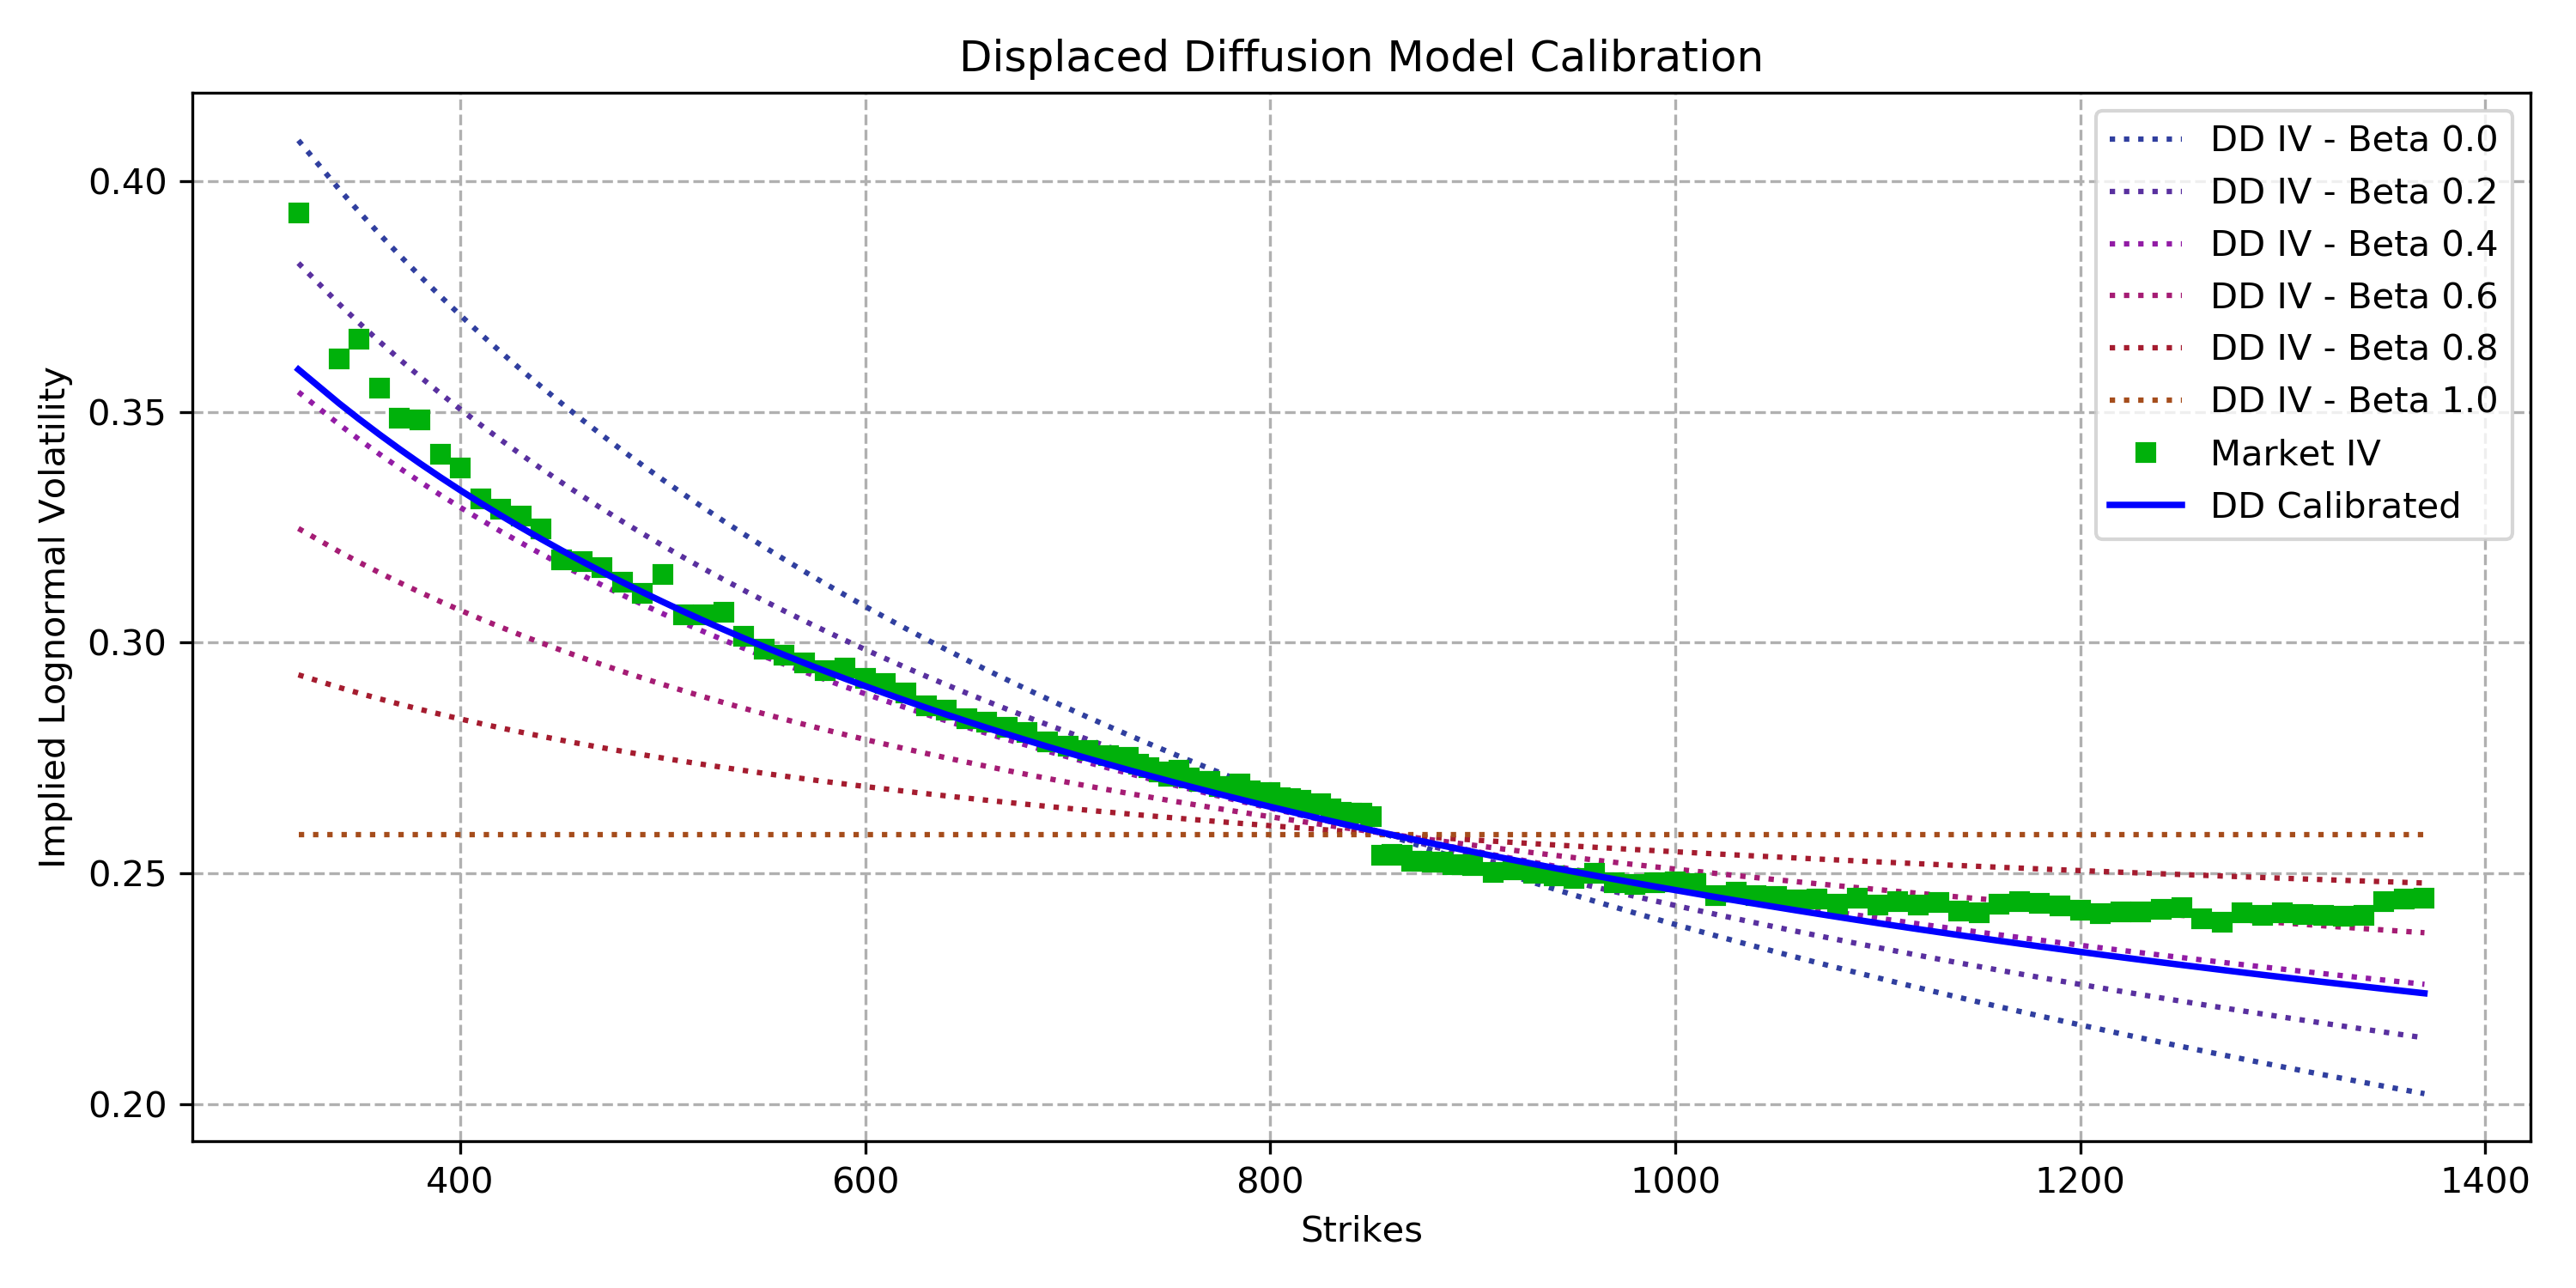
\includegraphics[width= \linewidth]{DD.png}
	%\caption{Displaced Diffusion Model Calibration}
\end{figure}
\noindent\\
Implied volatility from market prices were extracted using the Displaced Diffusion (DD) model with Beta=1, equivalent to the Black-76 Lognormal option pricing model, and the resulting implied volatilities plotted as ``Market IV".\\
\noindent\\
Differing values of Betas were input into the DD model to estimate which Beta parameter would most closely represent the implied volatility observed in the market. The main challenge in fitting the model was that in attempting to fit the IV of the lower strikes, we have to accept a larger deviation in the IV of the higher strikes, and vice versa. A least-squares method was used to find the Beta that would most closely fit market IV. This resulted in Beta parameters of approximately 0.3658.\\
\noindent\\
We note that while it does a sufficiently good job at matching ATM strike IVs, it gives a poor fit for the IVs for strikes at the extreme ends. The reason for this is that the market is pricing in a much higher IV value for lower strikes, and much lower IV value for higher strikes than these models suggest. This could partially be explained by behavioural reasons rooted in risk aversion, i.e. investors are willing to pay relatively high premiums for protection against large downside moves. Investors are also less willing to pay higher premiums for much higher strikes, and this could be due to the skew of historical returns (i.e. absence of sharp spikes in upside returns). We thus need a model that is able to incorporate all these additional factors, and so we turn to the SABR model. \\


\section{SABR Model}
\underline{Calibrated Results:}

\begin{itemize}
	\item Alpha: 0.9908
	\item Rho: -0.2851
	\item Nu: 0.3522
\end{itemize}

\begin{figure}[ht]
	\centering
	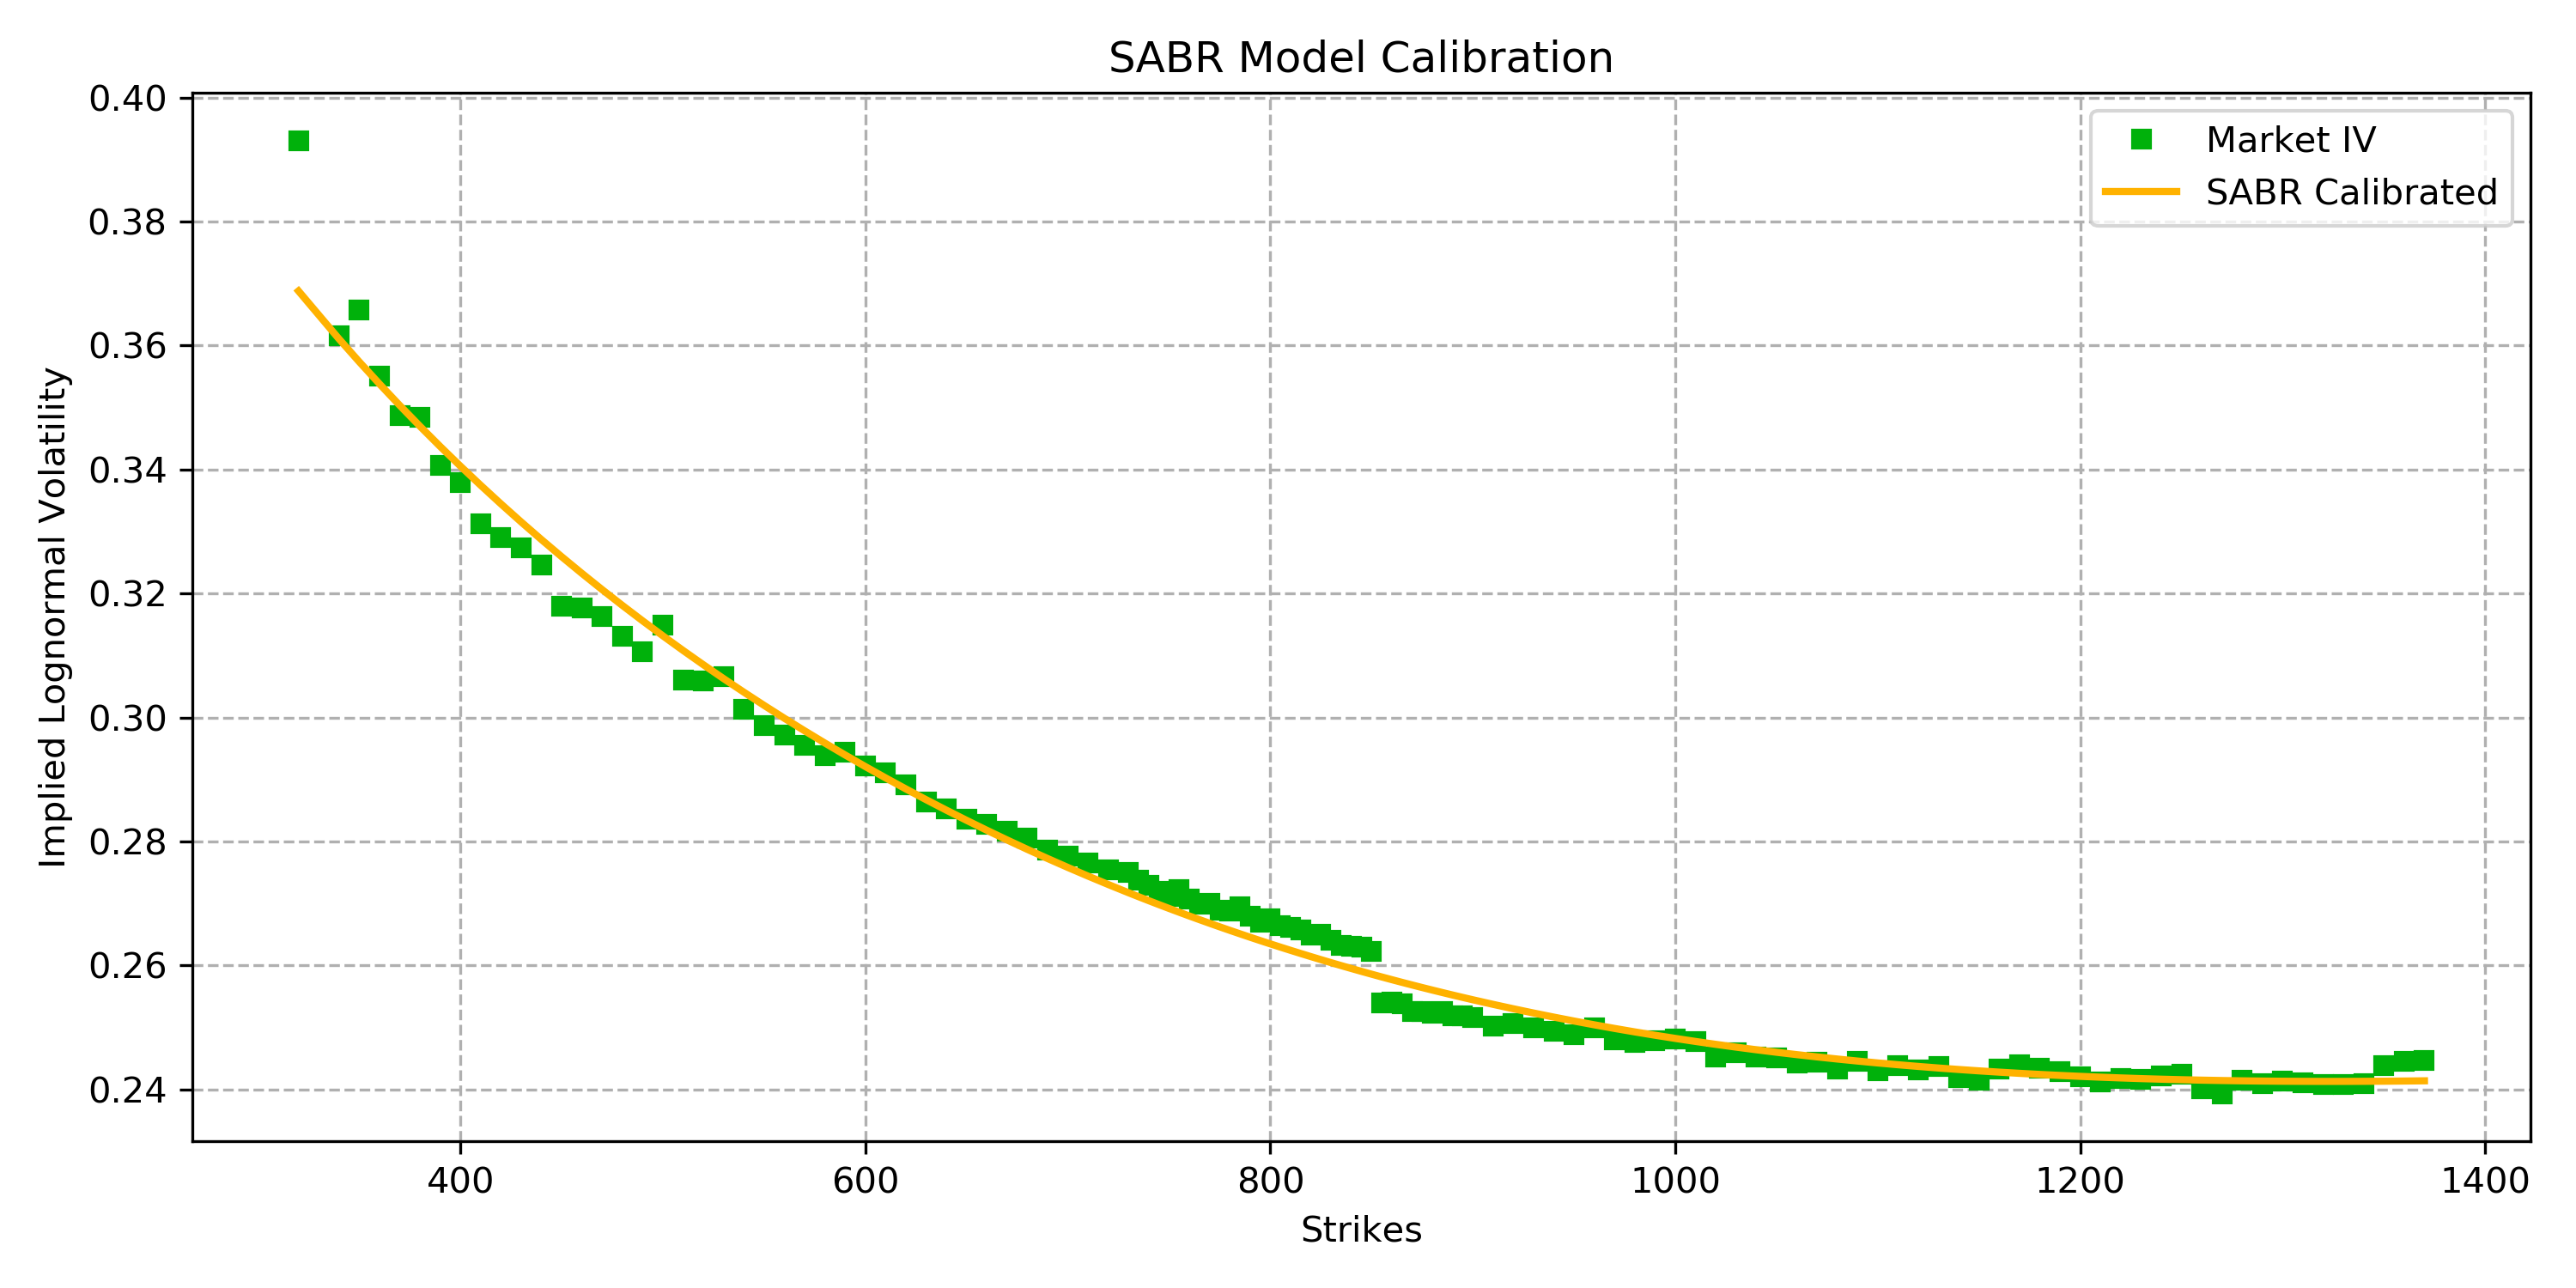
\includegraphics[width= \linewidth]{SABR.png}
	%\caption{SABR Model Calibration}
\end{figure}
\noindent\\
We calibrated the SABR model using the least squares method and obtained the following parameters of Alpha, Rho, and Nu, while keeping Beta fixed at 0.8. The calibrated SABR model fits the market IV very well, and this can be explained by the extra parameters which allow us to tweak the shape of the curve.\\


\begin{figure}[ht]
	\centering
	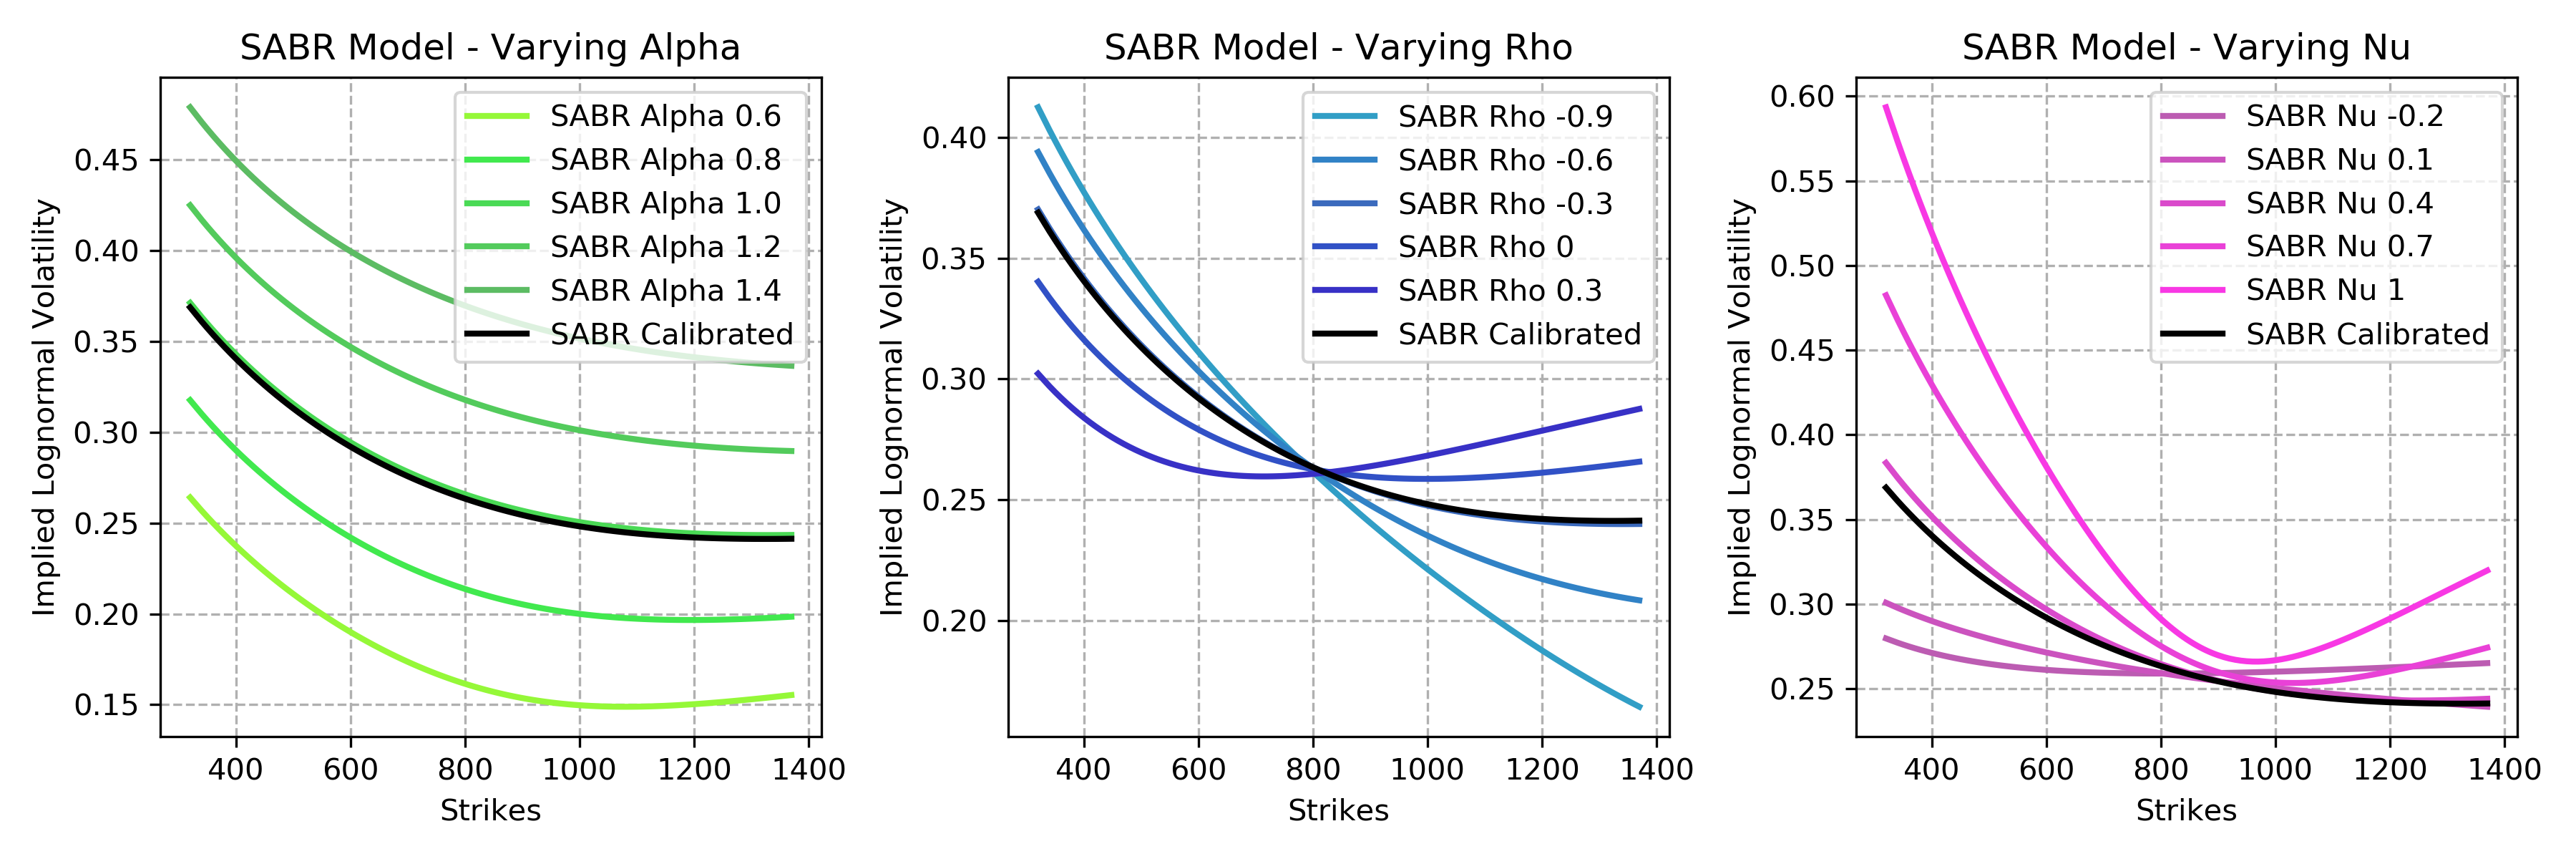
\includegraphics[width= \linewidth]{SABR-All.png}
	%\caption{SABR Model Calibration}
\end{figure}
\noindent\\
SABR Alpha adjusts for the height of the curve, and represents the constant of the volatility parameter. It can be seen as a baseline IV that is built into all the option prices. \\
\noindent\\
In the Black-Scholes model, the volatility term is deterministic, whereas in the SABR model, volatility of returns are modelled as being correlated with stock returns. SABR Rho adjusts for the skew in the distribution of stock returns. Decreasing the Rho adjusts for a more negative skew in stock returns. This allows us to increase the IVs of the lower strikes (OTM puts) to a higher IV than what the Black-Scholes model would suggest, and decrease the IVs of the higher strikes (OTM calls). Given that the calibrated correlation parameter is slightly negative, it implies that volatility increases when stock prices decrease. The adjustment also accounts for the behavioural factor that investors are usually more worried about downside risks than upside risks, and thus are willing to pay relatively higher prices for OTM lower strike puts as compared to similarly distant higher strikes OTM calls. \\
\noindent\\
SABR Nu adjusts for the volatility of volatility, and is proportionate to the degree of kurtosis of stock returns. A higher value of Nu increases the IV (and thus prices) of both calls and puts. This, coupled with a negative Rho value, leads to a much better curve that fits market prices and its corresponding expectations. \\
	
\section*{Part III: Static Replication}	
\setcounter{section}{0}
\section{Payoff function  $S^3_T+2.5 \log{S_T}+10.0 $}
\begin{minipage}[t]{0.5\textwidth}
	\begin{tcolorbox}[height=9cm,boxsep=5pt,arc=0pt,auto outer arc,colback=white,colframe=black]
		\noindent \textbf{The Black-Scholes model}\\ \\
		\noindent $\boldsymbol{S_T }\boldsymbol{= S_0 \exp\left[ \left(r-\frac{1}{2} \sigma^2 \right)T + \sigma W_T \right]}$\\ 
		where $W_T \sim N(0,T) \sim \sqrt{T} N(0,1) \sim \sqrt{T} x$.\\
		\noindent Given that: $\boldsymbol{\mathbb{E}[e^{\theta W_t}]=e^{\frac{\theta ^2}{2}t}}$ 
		\begin{align*}
		\mathbb{E}(S^3_T) &=\mathbb{E}(S^3_0 e^{[3(r-\frac{\sigma^2}{2})t+3\sigma W_t]})\\
		&=S^3_0 e^{[3(r-\frac{\sigma^2}{2})t]} \mathbb{E} [e^{3\sigma W_t}]\\
		&=S^3_0 e^{[3(r-\frac{\sigma^2}{2})t]} e^{\frac{9 \sigma^{2} t}{2}}\\
		&=S^3_0 e^{3t(r+\sigma^{2})}
		\end{align*}
		\noindent Given that: $\mathbb{E}(W_t)=0$
		\begin{flalign*}
		\mathbb{E}(\log{S_t})&=\mathbb{E}(\log{S_0})+\mathbb{E}((r-\frac{\sigma^2}{2})T+\sigma W_t)\\
		&=\log{S_0}+(r-\frac{\sigma^2}{2})T
		\end{flalign*}
	\end{tcolorbox}
\end{minipage}
\begin{minipage}[t]{0.5\textwidth}
\begin{tcolorbox}[height=9cm,boxsep=5pt,arc=0pt,auto outer arc,colback=white,colframe=black]
		\noindent \textbf{Contract Value:}
		\begin{flalign*}
		V_0 &= e^{-rT}\mathbb{E}(S^3_T+2.5\log{S_T}+10.0)\\
		&=e^{-rT}[\mathbb{E}(S^3_T)+2.5\mathbb{E}(\log{S_T})+10.0]\\
		&=e^{-rT}\{S^3_0 e^{3T(r+\sigma^{2})}\\
		&+2.5[\log{S_0}+(r-\frac{\sigma^{2}}{2})T]+10.0\}\\
		&=810237819.0000854
		\end{flalign*}\\
		\noindent \textbf{Additional Comments}\\ \\
		The underlying assumption of the Black=Scholes model is that implied volatilities are the same across all strikes. The At-The-Money option IV is used in the model, and so we use this value of sigma to value this contract.\\ \\
		 \\ \\
	\end{tcolorbox}
\end{minipage} \\ 
\begin{minipage}[t]{0.5\textwidth}
	\begin{tcolorbox}[height=9cm,boxsep=5pt,arc=0pt,auto outer arc,colback=white,colframe=black]
		\noindent \textbf{Bachelier Model}\\ \\
		$\boldsymbol{S_T} = S_0(1+\sigma W_T)$\\ 
		\noindent Given that $W_t\sim N(0,T)$, we can know that $\mathbb{E}(W_T)=0 \; , \;\mathbb{E}(W_T^2)=T,\textnormal{and} \mathbb{E}(W^3_T)=0$ 
		\begin{align*}
		\mathbb{E}(S^3_t)&=\mathbb{E}(S^3_0(1+\sigma W_t)^3)\\
		&=S^3_0\mathbb{E}(1+3\sigma W_t+3\sigma^2 W_t^2+\sigma^3 W_t^3)\\
		&=S^3_0(1+3\sigma t)
		\end{align*}
		\noindent And we need to calculate the $\mathbb{E}(\log{S_T})$ by numerical method, since:
		\begin{flalign*}
		&\mathbb{E}(\log{S_T}) = \mathbb{E}(\log{S_0}+\log{1+\sigma W_T})\\
		&=\log{S_0}+\frac{1}{\sqrt{2\pi}}\int_{-\infty}^{+\infty}{\log{(1+\sigma \sqrt{T}x)}e^{-\frac{x^2}{2}}dx}
		\end{flalign*}
	\end{tcolorbox}
\end{minipage}
\begin{minipage}[t]{0.5\textwidth}
	\begin{tcolorbox}[height=9cm,boxsep=5pt,arc=0pt,auto outer arc,colback=white,colframe=black]
		\noindent \textbf{Contract Value:}
		\begin{flalign*}
		V_0 &= e^{-rT}\mathbb{E}(S^3_T+\log{S_T}+10.0)\\
		&= e^{-rT}[S^3_0(1+3\sigma t)+\mathbb{E}(\log{S_T})+10.0]\\
		&=771273909.10267
		\end{flalign*}\\
		\noindent \textbf{Additional Comments}\\ \\
		The Bachelier model also uses a constant sigma, and so we use the same ATM option IV to value this contract. The At-The-Money option is most liquid amongst all strikes, and so it is the most representative.\\ \\
		 \\ \\
	\end{tcolorbox}
\end{minipage}\\ 
\begin{minipage}[t]{0.5\textwidth}
	\begin{tcolorbox}[height=5.5cm,boxsep=5pt,arc=0pt,auto outer arc,colback=white,colframe=black]
\subsection*{Static-replication}
\begin{flalign*}
&h(S_T)=S^3_T+2.5 \log{S_T}+10.0\\
&h'(S_T)=3S_T^2+\frac{2.5}{S_T}\\
&h''(S_T)=6S_T-\frac{2.5}{S_T^2}
\end{flalign*}
	\end{tcolorbox}
\end{minipage}
\begin{minipage}[t]{0.5\textwidth}
	\begin{tcolorbox}[height=5.5cm,boxsep=5pt,arc=0pt,auto outer arc,colback=white,colframe=black]
		\noindent \textbf{Contract Value:}
		\begin{align*}
		V_0 &= e^{-rT}h(F)+\int_{0}^{F} {h''(K)P(K)dK}\\
		&+ \int_{F}^{+\infty}{h''(K)C(K)dK}\\
		&=802756073.1462364
\end{align*}
P(K) and C(K) are Black76 Lognormal option prices with strikes across K. SABR sigma is used as the sigma input. 
	\end{tcolorbox}
\end{minipage}

\section{``Model-free" integrated   variance  $\sigma^2_{\textnormal{MF}}T=\mathbb{E}[\int_{0}^{T} {\sigma^2_t dt}]$}
\begin{minipage}[t]{0.5\textwidth}
	\begin{tcolorbox}[height=8cm,boxsep=5pt,arc=0pt,auto outer arc,colback=white,colframe=black]
\subsection{Black-Scholes model}
Using the Black-Scholes model, we can derive  
\begin{align*}
\mathbb{E}[\int_{0}^{T}{\sigma^2_T dt}]&=2\mathbb{E}[\int_{0}^{T}\frac{dS_t}{S_t}]-2\mathbb{E}[\log{\frac{S_t}{S_0}}]\\
&=2rT-2\mathbb{E}[(r-\frac{1}{2} \sigma^2 )T + \sigma W_T]\\
&=\sigma^{2}T
\end{align*}
We should use the ATM option implied volatility:  $\sigma^2_{\textnormal{MF}}=0.2582741$ \\ \\
	\end{tcolorbox}
\end{minipage}
\begin{minipage}[t]{0.5\textwidth}
	\begin{tcolorbox}[height=8cm,boxsep=5pt,arc=0pt,auto outer arc,colback=white,colframe=black]
\textbf{And given that}:
\begin{align*}
\mathbb{E}[\int_{0}^{T}{\sigma^2_T dt}]&=2e^{rT}\int_{0}^{F}{\frac{P(K)}{K^2}dK}\\
&+2e^{rT}\int_{F}^{+\infty}{\frac{C(K)}{K^2}dK}
\end{align*}
\subsection{Bachelier model}
Applying the Bachelier option pricer on P(K) and C(K), we obtain $\sigma^2_{\textnormal{MF}}=0.0920397$ 

\subsection{Static-replication}
Using the Static-replication approach, the Black76 Lognormal P(K) and C(K) values, along with SABR sigma, we obtain $\sigma^2_{\textnormal{MF}}=0.0755570$ 
	\end{tcolorbox}
\end{minipage}
\end{document}